\documentclass[border=5pt]{standalone}
\usepackage{tikz}
\usepackage{amsmath}
\usetikzlibrary{calc, positioning, arrows.meta, 3d}
\begin{document}
% Hanging mobile
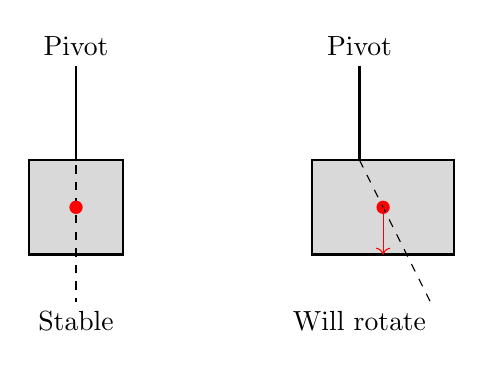
\begin{tikzpicture}[scale=1.2]
% Case 1: Stable
\draw[thick] (0,3) -- (0,2);
\draw[thick, fill=gray!30] (-0.5,1) rectangle (0.5,2);
\draw[dashed] (0,3) -- (0,0.5);
\fill[red] (0,1.5) circle (2pt);
\node[above] at (0,3) {Pivot};
\node[below] at (0,0.5) {Stable};

% Case 2: Unstable
\draw[thick] (3,3) -- (3,2);
\draw[thick, fill=gray!30] (2.5,1) -- (4,1) -- (4,2) -- (2.5,2) -- cycle;
\fill[red] (3.25,1.5) circle (2pt);
\draw[dashed] (3,2) -- (3.75,0.5);
\draw[red, ->] (3.25,1.5) -- (3.25,1);
\node[above] at (3,3) {Pivot};
\node[below] at (3,0.5) {Will rotate};
\end{tikzpicture}

\vspace{1cm}

% Leaning tower stability
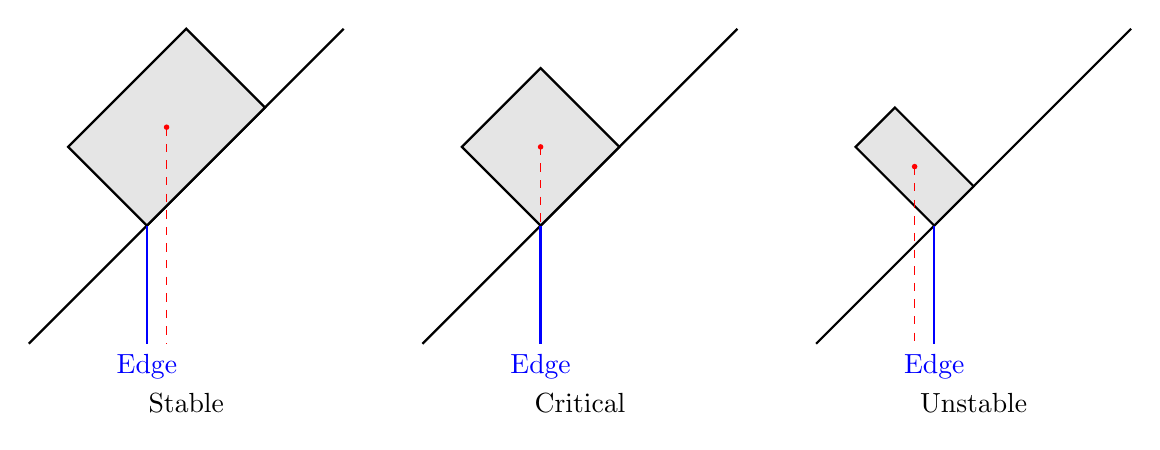
\begin{tikzpicture}[scale=1]
  \begin{scope}
% Tilted surface
\draw[thick] (0,0) -- (4,4);
% Block on surface
\draw[thick, fill=gray!20] (1.5,1.5) -- (3,3) -- (2,4) -- (0.5,2.5) -- cycle;
% Center of mass
\fill[red] (1.75,2.75) circle (1pt);
% Vertical line through C.M.
\draw[red, dashed] (1.75,2.75) -- (1.75,0);
% Edge of support
\draw[blue, thick] (1.5,1.5) -- (1.5,0) node[below] {Edge};
\node[below] at (2,-0.5) {Stable};
\end{scope}
\begin{scope}[xshift=5cm]
  % Tilted surface
\draw[thick] (0,0) -- (4,4);
% Block on surface
\draw[thick, fill=gray!20] (1.5,1.5) -- (2.5,2.5) -- (1.5,3.5) -- (0.5,2.5) -- cycle;
% Center of mass
\fill[red] (1.5,2.5) circle (1pt);
% Vertical line through C.M.
\draw[red, dashed] (1.5,2.5) -- (1.5,0);
% Edge of support
\draw[blue, thick] (1.5,1.5) -- (1.5,0) node[below] {Edge};
\node[below] at (2,-0.5) {Critical};
\end{scope}
\begin{scope}[xshift=10cm]
  % Tilted surface
\draw[thick] (0,0) -- (4,4);
% Block on surface
\draw[thick, fill=gray!20] (1.5,1.5) -- (2,2) -- (1,3) -- (0.5,2.5) -- cycle;
% Center of mass
\fill[red] (1.25,2.25) circle (1pt);
% Vertical line through C.M.
\draw[red, dashed] (1.25,2.25) -- (1.25,0);
% Edge of support
\draw[blue, thick] (1.5,1.5) -- (1.5,0) node[below] {Edge};
\node[below] at (2,-0.5) {Unstable};
\end{scope}
\end{tikzpicture}
\end{document}
